\documentclass[11pt]{article}
\usepackage[utf8]{inputenc}
\usepackage[french]{babel}
\usepackage{graphicx}
\usepackage[T1]{fontenc}
%\usepackage{amss}
\usepackage{amsmath}
\usepackage{amsfonts}
\usepackage{amssymb}

\newcommand\comment{}
\def\N{\mathbb N}
\def\R{\mathbb R}
\def\Q{\mathbb Q}
\def\Z{\mathbb Z}
\begin{document}
\title{PARTIEL I31, 2015 - CORRECTION}
\date{}\maketitle


{\bf 
J'ai noté 0 les réponses fausses, de même que les réponses 
confuses ou approximatives.
En effet, la langue naturelle est votre premier langage de programmation~: 
si vous ne savez pas écrire en français, vous ne saurez pas programmer.
La clarté, la précision, la concision de vos réponses sont donc essentielles.

De même, il faut savoir lire, c'est à dire comprendre ce que vous lisez.

Je rappelle qu'il faut lire l'énoncé...

Barême~: 3 points pour la première question, 1 point par question pour les autres. Le total fait 20 points.
}

\medskip
Tous vos documents sont autorisés, mais pas la copie de votre voisin.
N’écrivez aucun programme. Ecrivez lisiblement. Répondez aux questions
dans l’ordre, en indiquant le numéro de chaque question.

\section{Euclide et Bézout}

\smallskip

\begin{enumerate}
\item  En utilisant l'algorithme d'Euclide étendu, calculez le pgcd de 330 et 210 ainsi que les coefficients de Bezout:
$$u\in \Z, v\in \Z \ tels \ que \ 330u+210v=\mbox{PGCD}(330, 210)$$

Complétez le tableau ci-dessous. On rappelle que les coefficients $(u, v)$
de Bezout sont ceux pour lesquels $u^2 + v^2$ est le plus petit.

{\it 
Rappel: si $b=0$ alors $g=a$ et $u=1$. $v=0$ convient et donne la solution de norme minimale, mais tout $v\in \Z$ convient.
Si $b\neq 0$, alors soit $r=a\mod b$ et $q=a\div b$. Soit $u'$ et $v'$ tel que
$bu'+rv'=G$ ($G$ est le PGCD de $a$ et $b$). On en déduit~: $u=v'$, et $v=u'-qv'$.

\medskip
\begin{tabular}{|p{1.5cm}|p{1.5cm}|p{1.5cm}|p{1.5cm}|p{1.5cm}|p{1.5cm}|p{1.5cm}|}
\hline a & b & r=a\%b & q & pgcd(a,b) & u=v' & v=u'-qv'\\ 
\hline 
\hline  
330   &  210   & 120  & 1   & 30  & 2 & -3\\
\hline  
210 & 120   & 90  & 1 & 30  & -1 & 2 \\
\hline 
120 & 90   & 90  & 1 & 30  & 1  & -1 \\
\hline 
90 &  30  &  0 &  3  & 30  &  0 & 1  \\
\hline  
30 &  0  & --   & --    & 30  &  1 & 0  \\
\hline
\end{tabular}

En utilisant $k\in\Z$ au lieu de 0  pour valeur finale de $v$,  $u$ et $v$ deviennent des fonctions de $k$~:

\begin{tabular}{|p{1.5cm}|p{1.5cm}|p{1.5cm}|p{1.5cm}|p{1.5cm}|p{1.5cm}|p{1.5cm}|}
\hline a & b & r=a\%b & q & pgcd(a,b) & u(k) & v(k)\\
\hline
\hline  
330   &  210   & 120  & 1   & 30  & 2-7k & -3+11k\\
\hline  
210 & 120   & 90  & 1 & 30  & -1+4k & 2-7k \\
\hline
120 & 90   & 90  & 1 & 30  & 1-3k  & -1+4k \\
\hline 
90 &  30  &  0 &  3  & 30  &  k & 1-3k  \\
\hline  
30 &  0  & --   & --    & 30  &  1 & k  \\
\hline
\end{tabular}

La première ligne du tableau précédent permet de répondre à l aquestion suivante.
}

\item Donnez une formule avec un paramètre permettant de générer toutes les paires d'entiers  $(u, v)$ telles
que $330u+210v=\mbox{PGCD}(330, 210)$.

{\it 
La première ligne du tableau précédent nous donne~:
$$330 \times (u-7k) + 210\times (v+11k) = PGCD(330, 210)=30 $$
ou encore~:
$$330 \times (2-7k) + 210\times (-3+11k) = PGCD(330, 210)=30 $$

Autrement dit~: 
$$u_k=u-k(b/pgcd)=u-7k\;  et \; v_k=u+k(a/pgcd)=v+11k$$

On obtient sur l'exemple:
}


\medskip
\begin{tabular}{|p{2cm}|p{2cm}|p{2cm}||p{2cm}|p{2cm}|}
\hline k & u & v & au+bv & $u^2+v^2$\\ 
\hline -4 & 30 & -47 & 30 & 3109\\ 
\hline -3 & 23 & -36 & 30 & 1825\\ 
\hline -2 & 16 & -25 & 30 & 881\\ 
\hline -1 & 9 & -14 & 30 & 277\\ 
\hline 0 & 2 & -3 & 30 & 13\\ 
\hline 1 & -5 & 8 & 30 & 89\\ 
\hline 2 & -12 & 19 & 30 & 505\\  
\hline 3 & -19 & 30 & 30 & 1261\\ 
\hline 4 & -26 & 41 & 30 & 2357\\ 
\hline
\end{tabular}

\end{enumerate}



\section{Quizz}

\begin{enumerate}
\item Citez deux problèmes indécidables en informatique.

\emph{La terminaison d’un algorithme (ou d’une machine de Turing), l’égalité de deux nombres réels (ou complexes), l’égalité de deux fonctions (par exemple de N dans N). }



\item  Quand dit-on qu'un problème est difficile en informatique.

{\it Quand aucun algorithme en temps polynomial permettant de résoudre ce problème n’est connu\footnote{Ce qui ne prouve pas qu'il n'en existe pas...}.

Quelques réponses fausses~: 

- quand il existe un algorithme en temps exponentiel. Or il existe un algorithme  en temps exponentiel pour le tri, tel que générer toutes les permutations possibles. 

- quand il n'existe qu'un ou des  algorithmes en temps non polynomial. Le problème avec cette réponse est~: pour certains problèmes, il n'y a pas d'algorithme
connu qui marche en temps polynomial, mais cela ne prouve pas qu'il n'en existe pas. Ainsi, personne ne sait prouver l'inexistence d'algorithme en temps polynomial pour résoudre les problèmes de la classe NP. 
}

\item  Citez deux problèmes solubles en informatique, mais difficiles.


\emph{Résoudre un problème SAT (où un solveur SAT est un programme qui décide automatiquement si une formule de logique
propositionnelle est satisfaisable). Trouver un chemin ou un circuit hamiltonie
n (passant par tous les sommets dans un graphe). Trouver une clique
ou un stable de taille maximale ou de taille fixée. Plus généralement, résoudre un problème de la classe NP. Factoriser un très grand entier est aussi un problème difficile, car aucun algorithme en temps polynomial n'est connu aujourd'hui. De même pour le problème du logarithme discret: résoudre $a^x=b \mod p$ où $p$ est un entier premier.}





\item Donnez deux algorithmes efficaces pour trier des nombres en utilisant
des comparaisons. Indiquez la complexité (en nombre de comparaisons)
de ces deux algorithmes. 
\begin{itemize}
\item  \emph{tri par fusion (mergesort, $O(n*log(n)$)}
\item  \emph{tri par tas (heapsort, $O(n*log(n)$)}
 \item  \emph{tri rapide (quicksort, en moyenne complexité en $O(n*log(n)$).}
\end{itemize}

\item   Donnez le nom de trois algorithmes calculant les plus courts chemins dans un graphe.

\emph{Dijkstra, Floyd, Ford (ou Ford-Bellman), Dantzig, Warshall, pseudo produit matriciel: $(AB)_{l,c}= min_k (A_{lk} + B_{kc})$.}

\end{enumerate}

\section{Ordonnancement}

\begin{center}
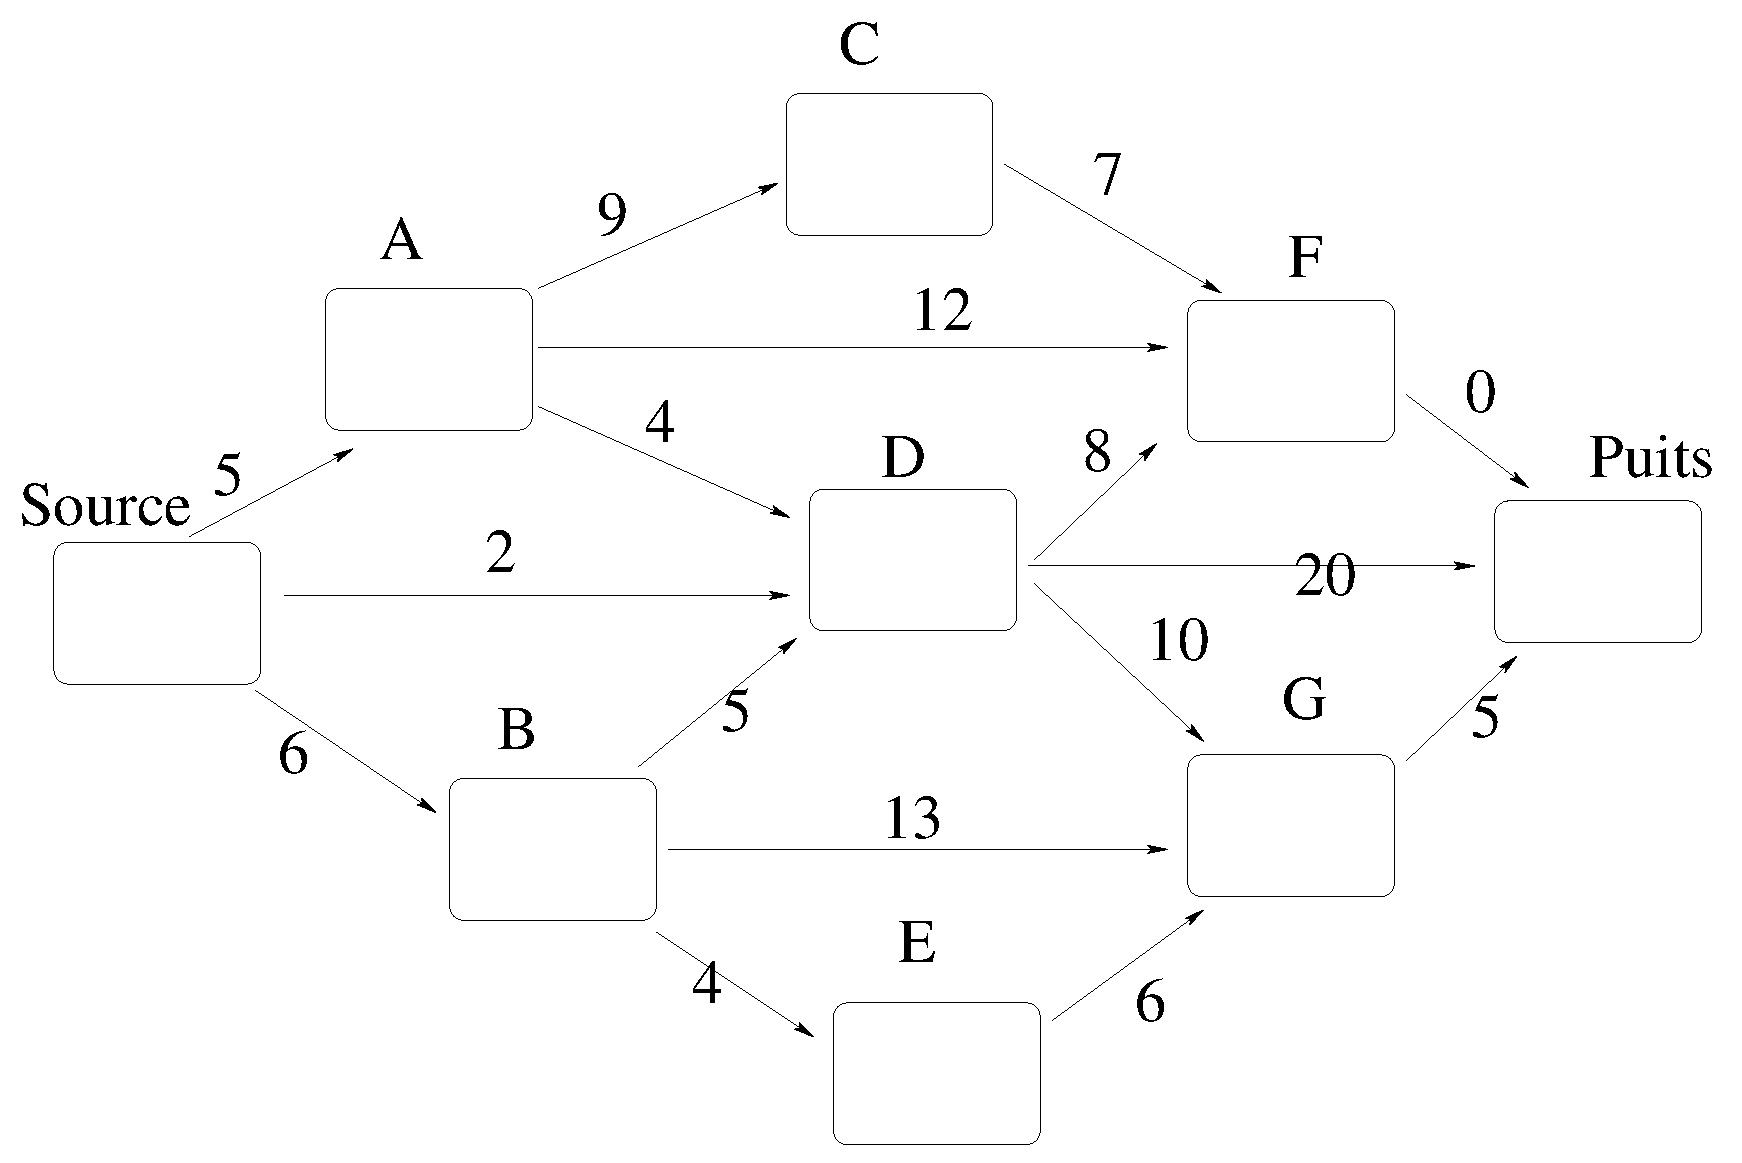
\includegraphics[width=0.95\linewidth]{critique.eps}
\end{center}


Etant donnée la description des tâches donnée ci-dessus: 

\begin{enumerate}

\item 
En calculant de SOURCE vers PUIT, complétez les dates au plus tôt (comme par exemple 0- et 5-).


Puis en calculant de  PUIT vers SOURCE, complétez les dates au plus tard (comme par exemple -0 et -7).

Soulignez le chemin critique.

\begin{center}
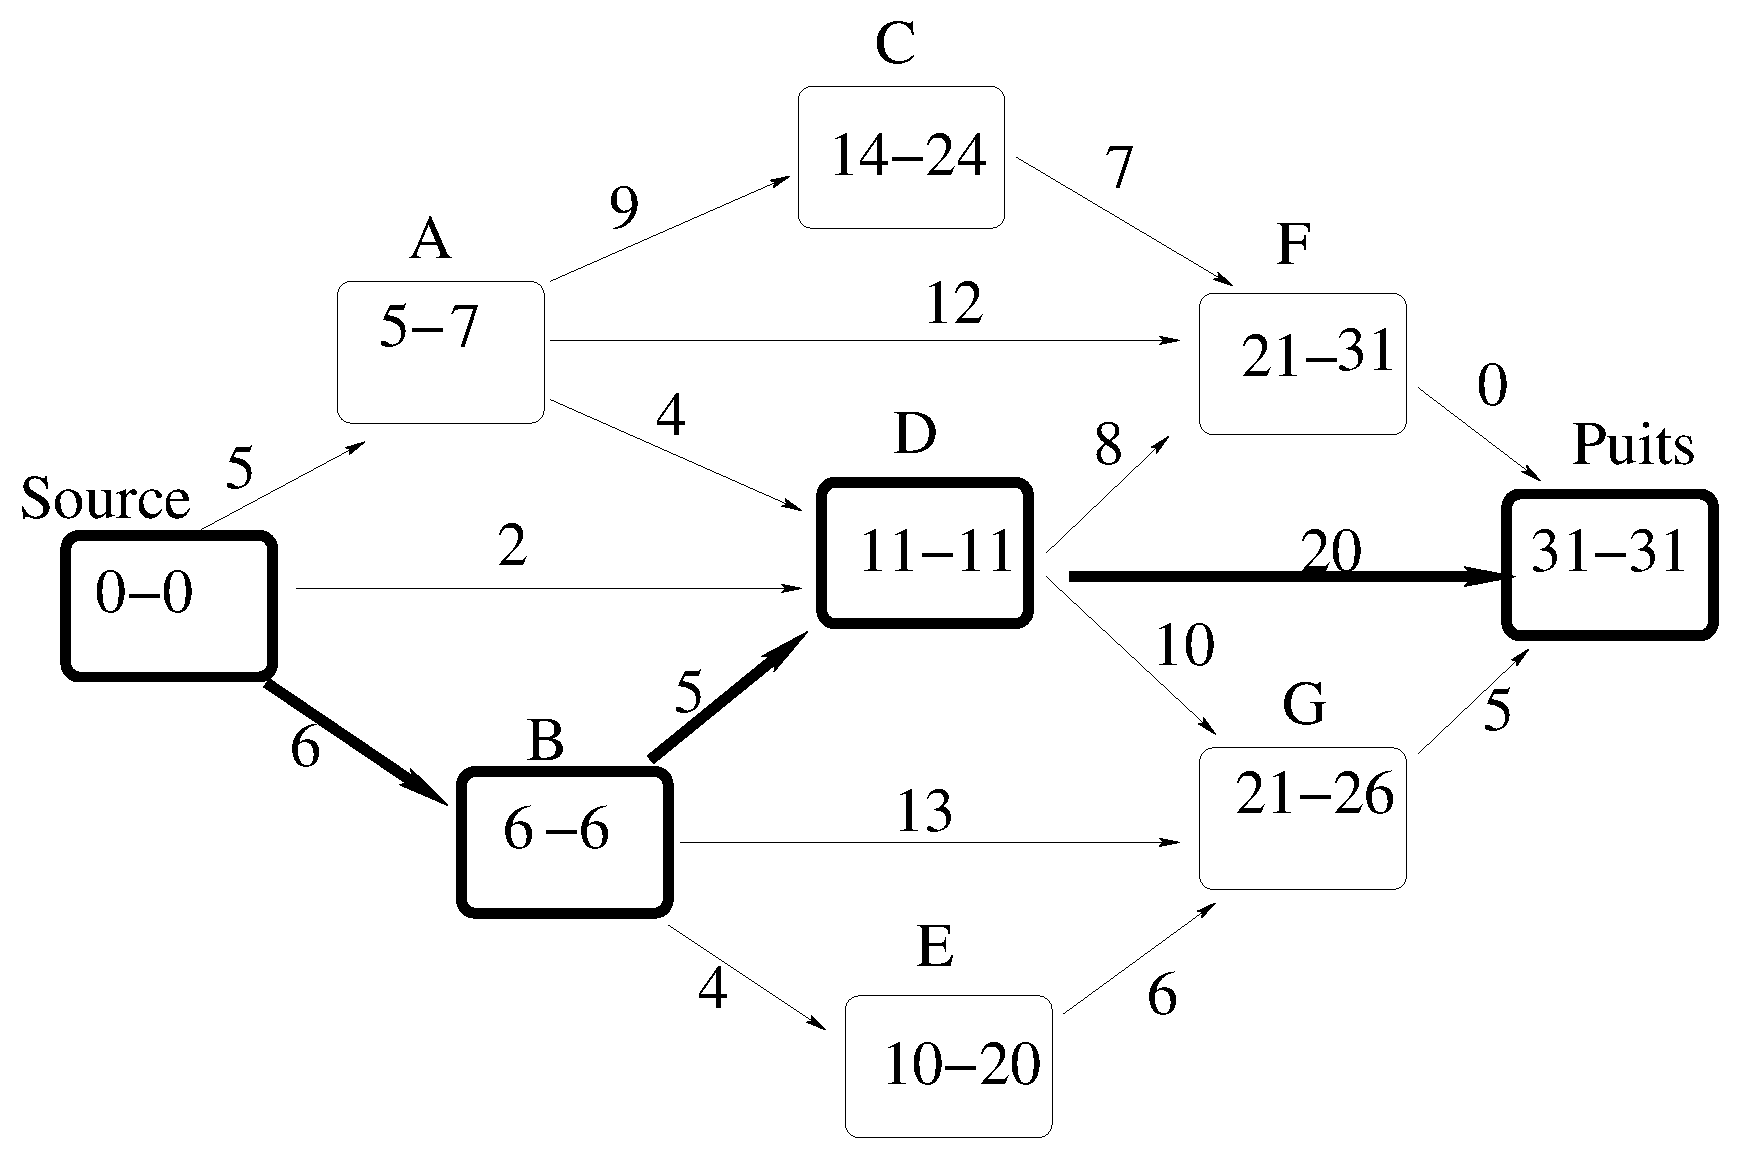
\includegraphics[width=0.95\linewidth]{critique_solution.eps}
\end{center}

%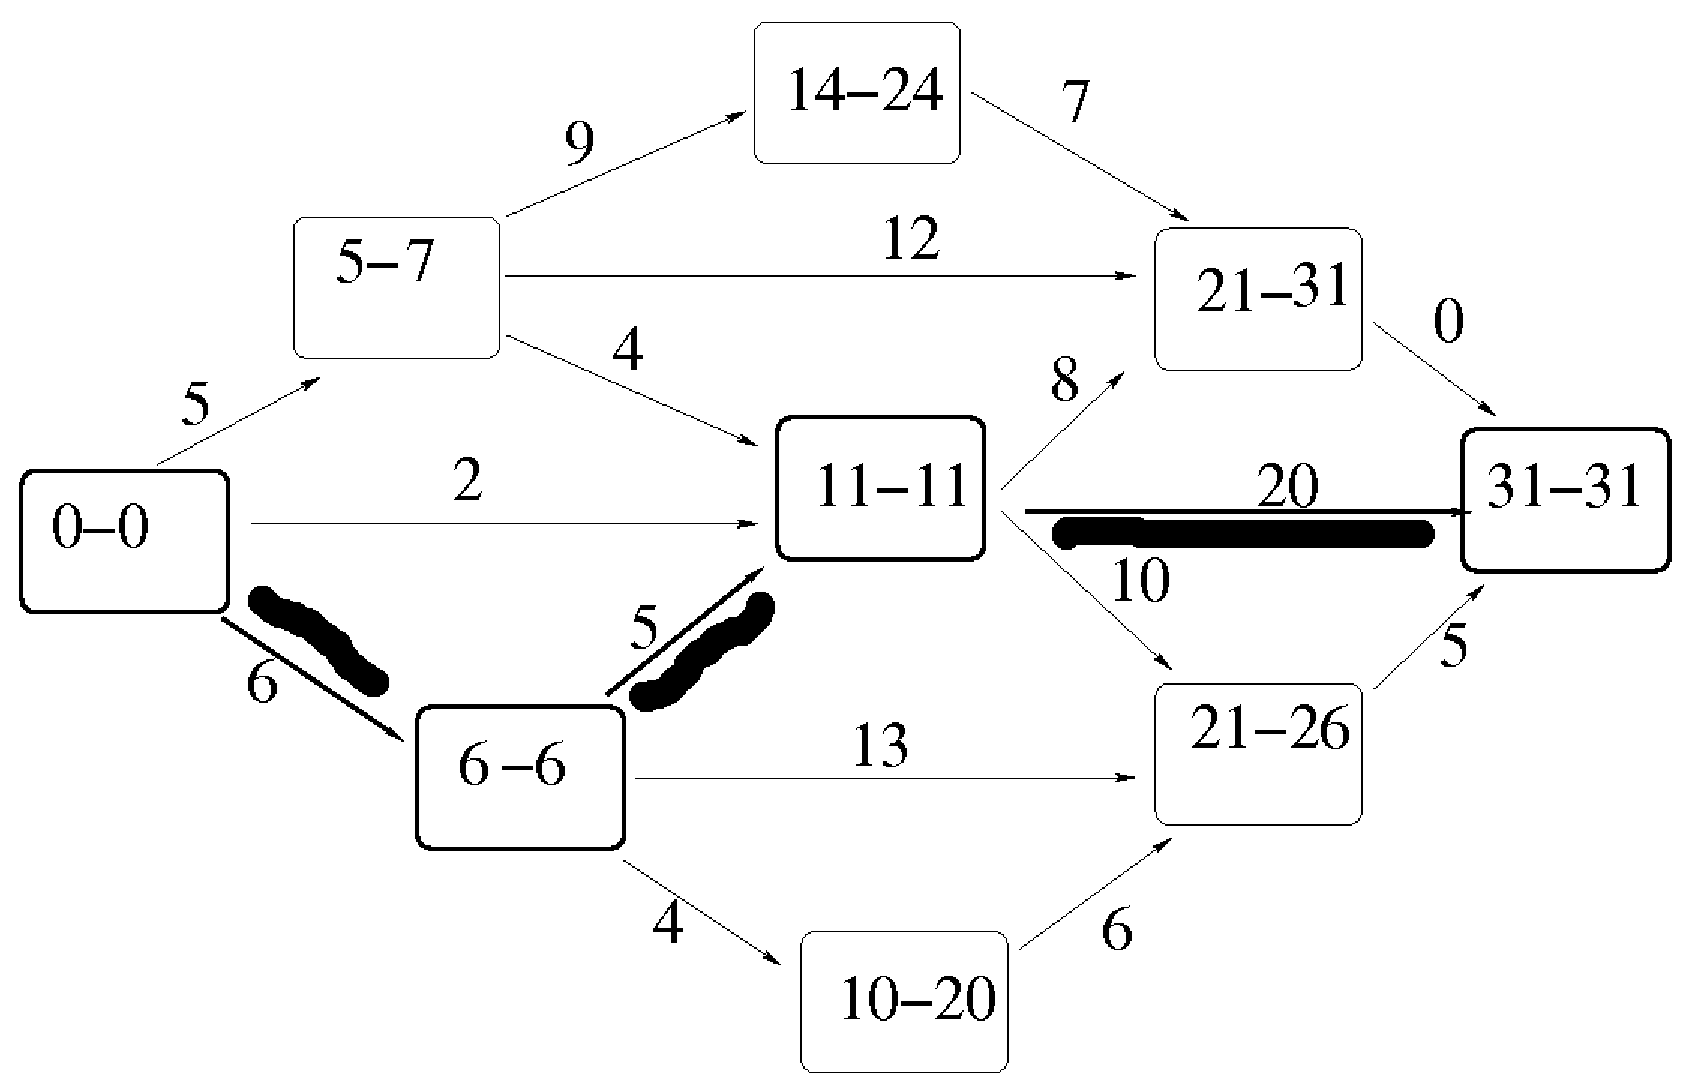
\includegraphics[width=0.95\linewidth]{critique_solutionCHEMIN.eps}



\item Que faire si le graphe a plusieurs sommets sources (ou puits) ?

\emph{Si un graphe a plusieurs sources, on peut ajouter une source virtuelle
$\Omega$  reliée à toutes les sources $s$  par un arc $\Omega\rightarrow s$  de durée nulle.}

 \emph{De même pour un graphe ayant plusieurs puits.
Chaque  puits $p$ est relié à un sommet terminal $P$  par un arc
$s\rightarrow P$ de durée nulle. 
}

\item  Vous pouvez supposer que le graphe est acyclique, qu'il a un seul sommet source, un seul sommet puits, et que les durées sur les arcs sont non négatives.
Donnez la définition, en français, de la date au plus
tôt. Prévoyez bien tous les cas : sommet avec ou sans arc entrant ou
sortant.

%\emph
{\it
$s$ est la source  $\Rightarrow \mbox{Tôt}(s) = 0$

Sinon~:
$$\mbox{Tôt}(s)= \max_{r:\; r\rightarrow s} \mbox{Tôt}(r)+ C(r\rightarrow s)$$
c'est à dire le maximum, pour tous les
sommets $r$ tels qu'il existe un arc $r\rightarrow s$,  des 
$\mbox{Tôt}(r)+\mbox{Durée}(r\rightarrow s)$.

Remarque~: la date au plus tôt de $s$ est la longueur du chemin le plus {\bf long} de la source jusqu'à $s$, et non pas le chemin le plus court. Ici, ce problème est facile car le graphe est acyclique~; rappelons que calculer le chemin (acyclique) le plus long dans un graphe avec cycle  est difficile~: le chemin hamiltonien est un cas particulier de ce problème où tous les coûts sont égaux (à 1 par exemple).
}

\item   Donnez la définition, en français, de la date au plus tard. Prévoyez bien tous les cas.

%\emph
{\it
$s$ est le puits  $\Rightarrow \mbox{Tard(s)= Tôt}(s)$.

Sinon~:
$$\mbox{Tard}(s)=\min_{t:\; s\rightarrow t} \mbox{Tard}(t) - \mbox{Durée}(s\rightarrow t)$$
}

\item   Quand un sommet est-il critique~?

\emph{Lorsque ses dates au plus tôt et au plus tard sont identiques.}
\end{enumerate}

\section{Dessinez le graphe d'un jeu de Nim}
Deux joueurs jouent à tour de rôle (Albert commence, Bertrand joue en second). Sur la table, il y a trois tas de pions~:
deux tas de 2 pions, et un tas de 1.

\smallskip
Chacun des joueurs choisit un tas (non vide) et  un seul,
et en retire un nombre entier  non nul  de pions~; il peut retirer  tous les pions du tas s'il le souhaite.

\smallskip
Le premier joueur qui ne peut plus retirer de pions
a perdu, ou, le premier joueur qui enlève tous les pions restant dans le dernier tas a gagné. 

\medskip
Vous utiliserez une représentation des états par niveaux: le niveau $n$ contient les états où la somme des nombres de pions vaut $n$ ($0 \le n \le 6 $). Un seul des états équivalents est représenté ($(2, 1, 1)=(1, 2, 1)=(1, 1, 2)$) et les $0$ inutiles sont éliminés.

Par exemple le niveau 2 contient
les états $(2)$ et $(1, 1)$. 

\medskip
Un sommet est gagnant si et seulement si le joueur qui y arrive peut toujours gagner, quels que soient les coups joués par l'adversaire.
Un sommet est perdant si et seulement si il n'est pas gagnant.


 \begin{enumerate}
\item  Le schéma fourni ne contient que les niveaux 0, 1, 2. Ajoutez les 4 états
manquants.

\emph{Voir Figure ci-dessous.}

\item  Sur le graphe, dessinez les arcs de tous les coups possibles ; il y a 16
arcs en tout ; chaque état est représenté par un sommet ; un arc va d’un
sommet $s$ à un sommet $t$ quand il est possible de passer en un coup de
$s$ à $t$.


\emph{Voir Figure ci-dessous.}


\item Marquez chaque sommet $G$ s’il est gagnant et $P$ s’il est perdant. Epaississez le contour des sommets gagnants.


\emph{Voir Figure ci-dessous.}


\item  Quel joueur, Albert ou Bertrand, est sûr de gagner, s'il joue intelligemment, bien sûr~?

\emph{Albert est sûr de gagner s'il enlève le pion isolé. }

\item Décrivez l'algorithme que vous avez utilisé pour marquer les sommets  $G$ ou $P$.

\emph{La position finale est gagnante. Il faut "remonter" vers la position initiale avec :}
\begin{itemize}
\item \emph{une position ayant au moins un arc  vers une position gagnante est perdante}
\item \emph{dit autrement, une position dont tous les arcs sortants mènent à une position perdante est gagnante}
\end{itemize}

\item  Dans un graphe orienté acyclique (c'est le cas ici), un noyau $N$ est 
un sous-ensemble de sommets du graphe tel que~: si $s$ est dans $N$, tous ses voisins sont hors de $N$~; si $s$ est hors de $N$, il existe au moins un arc vers un sommet $t$ qui se trouve dans $N$. 

Quel est le lien avec le problème précédent~? 

\emph{Les positions gagnantes forment un noyau.}

\end{enumerate}

\bigskip

\begin{center}
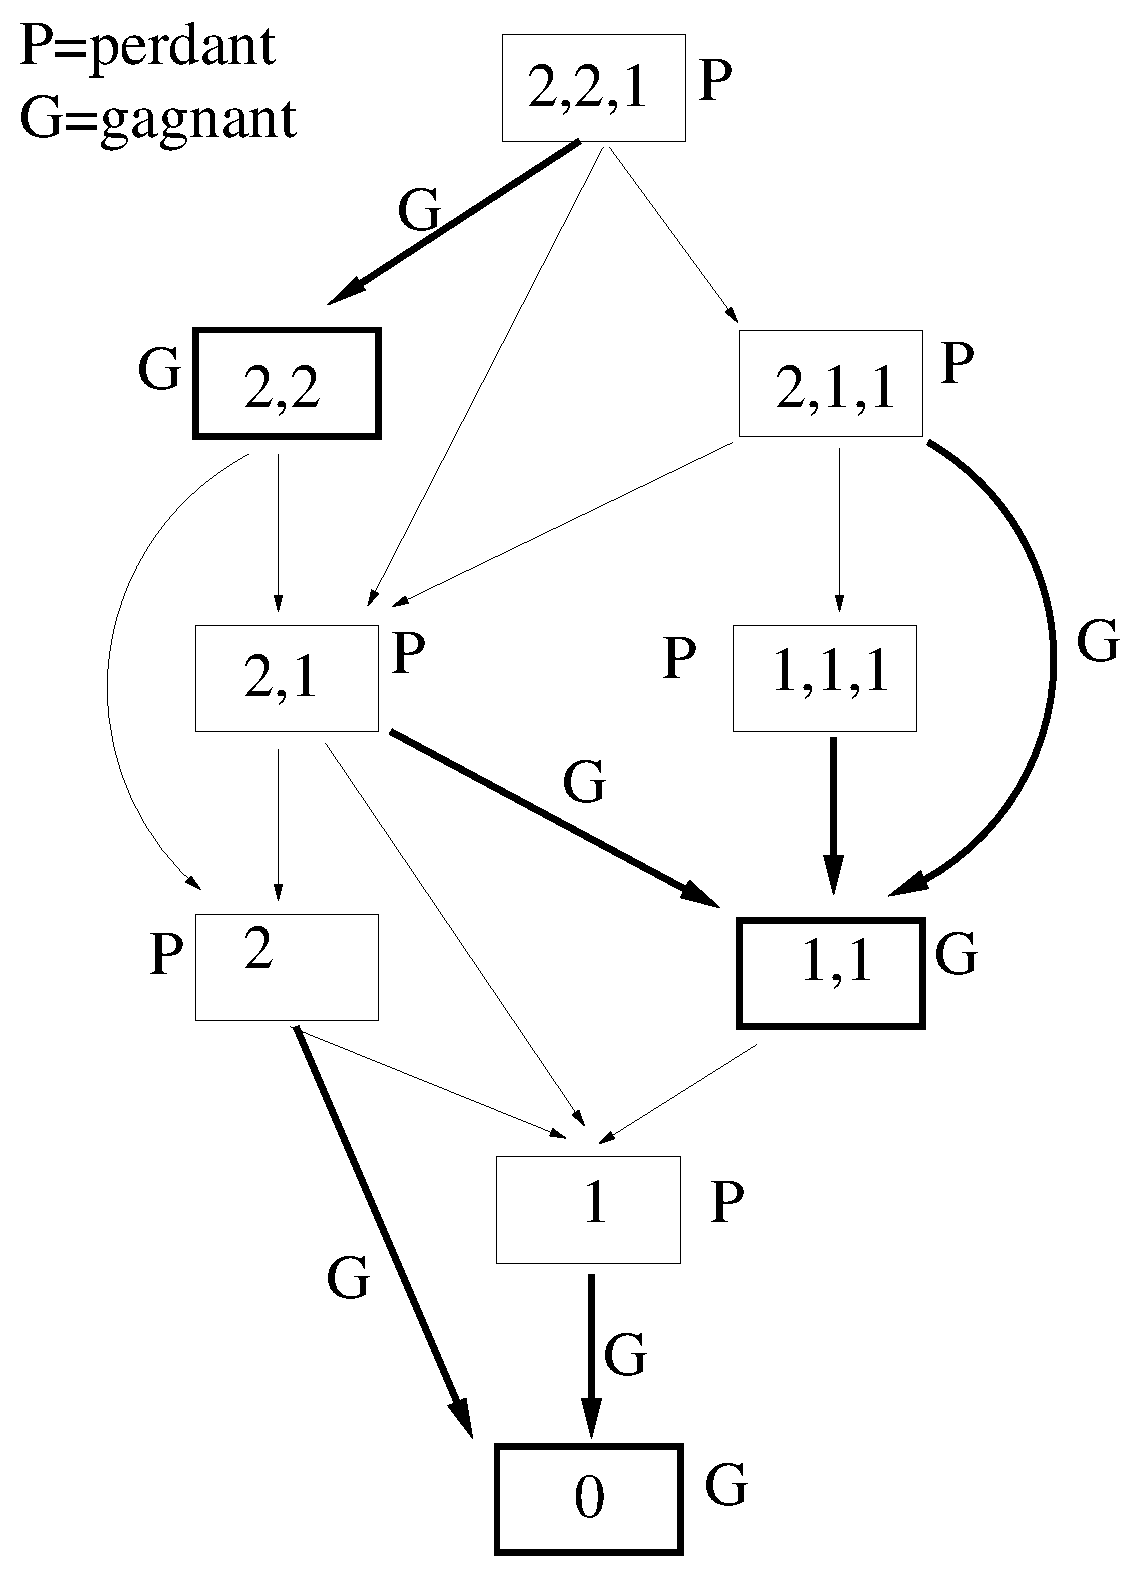
\includegraphics[width=0.75\linewidth]{nim.eps}
\end{center}
Remarque sur le dessin du graphe~: il est bien précisé dans l'énoncé de dessiner niveau par niveau, et qu'un seul sommet doit être dessiné quand plusieurs états sont équivalents~: $(2,1,1)=(1,2,1)=(1,1,2)$, etc.

\end{document}
